\documentclass[11pt,a4paper]{article}

% Packages
\usepackage[margin=2.5cm]{geometry}
\usepackage{microtype}
\usepackage{graphicx}
\usepackage{tikz}
\usetikzlibrary{shapes,arrows.meta,positioning,calc,fit,backgrounds,shadows.blur,decorations.pathmorphing,decorations.pathreplacing}
\usepackage{colortbl}
\usepackage{enumitem}
\usepackage{booktabs}
\usepackage{longtable}
\usepackage{hyperref}
\usepackage{xcolor}
\usepackage{fancyhdr}
\usepackage{titlesec}
\usepackage[most]{tcolorbox}
\usepackage{multicol}
\usepackage{amsmath,amssymb}
\usepackage{multirow}
\usepackage{setspace}
\usepackage{fontawesome5}
\usepackage{listings}

% Spacing
\setlength{\parskip}{3pt plus 1pt minus 1pt}
\setlength{\parindent}{0pt}

% Colors
\definecolor{primary}{HTML}{0E4D64}
\definecolor{secondary}{HTML}{137177}
\definecolor{accent}{HTML}{C84B31}
\definecolor{lightbg}{HTML}{E8F6F3}
\definecolor{defbg}{HTML}{FDF2E9}
\definecolor{greenhl}{HTML}{2E8B57}
\definecolor{purplehl}{HTML}{6C5B7B}
\definecolor{codebg}{HTML}{F4F6F7}

% Hyperref
\hypersetup{colorlinks=true, linkcolor=primary, urlcolor=secondary, citecolor=primary}

% Code listings style
\lstset{
  backgroundcolor=\color{codebg},
  basicstyle=\ttfamily\small,
  keywordstyle=\color{primary}\bfseries,
  stringstyle=\color{greenhl},
  commentstyle=\color{gray},
  breaklines=true,
  frame=l,
  framerule=2pt,
  rulecolor=\color{secondary!40},
  xleftmargin=8pt,
  framexleftmargin=6pt,
  aboveskip=6pt,
  belowskip=6pt
}

% Header/Footer
\pagestyle{fancy}
\fancyhf{}
\fancyhead[L]{\small\textcolor{primary}{\textbf{IT Project Management --- Data Science for BSIT}}}
\fancyhead[R]{\small\textcolor{primary}{Lecture Handout}}
\fancyfoot[C]{\small\thepage}
\renewcommand{\headrulewidth}{0.5pt}
\renewcommand{\footrulewidth}{0.3pt}

% Section formatting
\titleformat{\section}{\Large\bfseries\color{primary}}{\thesection}{0.6em}{}[\vspace{2pt}\titlerule]
\titleformat{\subsection}{\large\bfseries\color{secondary}}{\thesubsection}{0.5em}{}
\titleformat{\subsubsection}{\normalsize\bfseries\color{primary}}{\thesubsubsection}{0.5em}{}
\titlespacing*{\section}{0pt}{14pt}{8pt}
\titlespacing*{\subsection}{0pt}{10pt}{5pt}

% Custom boxes
\newtcolorbox{definitionbox}[1][] {
  enhanced, breakable,
  colback=defbg, colframe=orange!60!black,
  colbacktitle=orange!70!black, coltitle=white,
  title={\faIcon{book}~#1}, fonttitle=\bfseries,
  boxrule=0pt, leftrule=4pt, arc=2pt,
  shadow={1mm}{-1mm}{0mm}{black!15},
  top=4pt, bottom=4pt, left=8pt, right=8pt
}
\newtcolorbox{conceptbox}[1][] {
  enhanced, breakable,
  colback=lightbg, colframe=secondary,
  colbacktitle=secondary, coltitle=white,
  title={\faIcon{lightbulb}~#1}, fonttitle=\bfseries,
  boxrule=0pt, leftrule=4pt, arc=2pt,
  shadow={1mm}{-1mm}{0mm}{black!15},
  top=4pt, bottom=4pt, left=8pt, right=8pt
}
\newtcolorbox{alertbox}[1][] {
  enhanced, breakable,
  colback=red!4, colframe=accent,
  colbacktitle=accent, coltitle=white,
  title={\faIcon{exclamation-triangle}~#1}, fonttitle=\bfseries,
  boxrule=0pt, leftrule=4pt, arc=2pt,
  shadow={1mm}{-1mm}{0mm}{black!12},
  top=3pt, bottom=3pt, left=8pt, right=8pt
}
\newtcolorbox{examplebox}[1][] {
  enhanced, breakable,
  colback=green!4, colframe=greenhl,
  colbacktitle=greenhl, coltitle=white,
  title={\faIcon{code}~#1}, fonttitle=\bfseries,
  boxrule=0pt, leftrule=4pt, arc=2pt,
  shadow={1mm}{-1mm}{0mm}{black!12},
  top=3pt, bottom=3pt, left=8pt, right=8pt
}

\begin{document}

% Title
\begin{center}
\vspace*{0.5cm}
{\Huge\bfseries\textcolor{primary}{IT Project Management}}\\[8pt]
{\Huge\bfseries\textcolor{primary}{AI-Enhanced Delivery and Control}}\\[16pt]
{\color{secondary}\rule{0.68\textwidth}{1.5pt}}\\[12pt]
{\Large\textsc{BSIT Lecture Handout}}\\[6pt]
{\large\textcolor{gray!70!black}{Course: Data Science \quad Program: BSIT}}\\[8pt]
{\normalsize\textcolor{gray!70!black}{Planning \textbullet\ Estimation \textbullet\ Risk \textbullet\ Agile Delivery \textbullet\ AI Decision Support}}
\vspace{0.3cm}
\end{center}

\tableofcontents
\newpage

%=============================================================
\section{Introduction to IT Project Management}
%=============================================================

\begin{definitionbox}[IT Project Management]
IT project management is the structured planning, execution, monitoring, and closure of technology-related work so that a defined product, service, or system is delivered within agreed scope, time, cost, quality, and risk constraints.
\end{definitionbox}

\begin{conceptbox}[Why This Matters in a Data Science Course]
Data science projects are still projects. They require scope definition, stakeholder communication, resource planning, schedules, budgets, quality control, and risk management. What changes in this handout is the use of artificial intelligence to improve how managers forecast work, detect risk, summarize progress, and support decisions.
\end{conceptbox}

\subsection{Project, Program, and Operations}

\begin{itemize}[leftmargin=*]
  \item \textbf{Project:} Temporary effort with a start and end date that produces a unique output.
  \item \textbf{Program:} Group of related projects managed together for coordinated benefit.
  \item \textbf{Operations:} Ongoing repetitive work that keeps an organization running.
\end{itemize}

\subsection{Typical IT Project Goals}

\begin{itemize}[leftmargin=*]
  \item Deliver a software application or platform.
  \item Implement infrastructure, cybersecurity, or data solutions.
  \item Improve service quality, automation, or reporting.
  \item Meet regulatory, business, or academic requirements.
\end{itemize}

\subsection{The Triple Constraint and Beyond}

\begin{center}
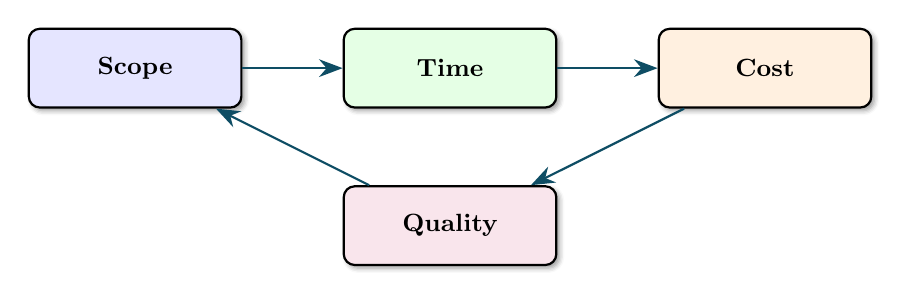
\begin{tikzpicture}[
  box/.style={rectangle, draw, thick, rounded corners=4pt, minimum width=2.7cm, minimum height=1cm, align=center, font=\small\bfseries,
    blur shadow={shadow blur steps=4, shadow xshift=0.4mm, shadow yshift=-0.4mm}},
  arr/.style={-{Stealth[length=3mm]}, thick, primary}
]
  \node[box, fill=blue!10] (scope) at (0,0) {Scope};
  \node[box, fill=green!10] (time) at (4,0) {Time};
  \node[box, fill=orange!12] (cost) at (8,0) {Cost};
  \node[box, fill=purple!10] (quality) at (4,-2) {Quality};

  \draw[arr] (scope) -- (time);
  \draw[arr] (time) -- (cost);
  \draw[arr] (cost) -- (quality);
  \draw[arr] (quality) -- (scope);
\end{tikzpicture}
\end{center}

\begin{conceptbox}[Management Reality]
Modern project management goes beyond the classic scope-time-cost triangle. It also considers quality, stakeholder satisfaction, business value, security, sustainability, and team capacity. AI can help observe these dimensions, but it does not remove the need for managerial judgment.
\end{conceptbox}

%=============================================================
\section{The Project Lifecycle and Management Foundations}
%=============================================================

\subsection{Project Lifecycle}

\begin{center}
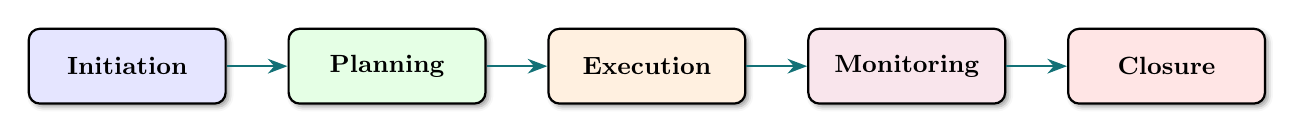
\begin{tikzpicture}[
  phase/.style={rectangle, draw, thick, rounded corners=4pt, minimum width=2.5cm, minimum height=0.95cm, align=center, font=\small\bfseries,
    blur shadow={shadow blur steps=3, shadow xshift=0.4mm, shadow yshift=-0.4mm}},
  arr/.style={-{Stealth[length=2.5mm]}, thick, secondary}
]
  \node[phase, fill=blue!10] (start) at (0,0) {Initiation};
  \node[phase, fill=green!10] (plan) at (3.3,0) {Planning};
  \node[phase, fill=orange!12] (exec) at (6.6,0) {Execution};
  \node[phase, fill=purple!10] (monitor) at (9.9,0) {Monitoring};
  \node[phase, fill=red!10] (close) at (13.2,0) {Closure};

  \draw[arr] (start) -- (plan);
  \draw[arr] (plan) -- (exec);
  \draw[arr] (exec) -- (monitor);
  \draw[arr] (monitor) -- (close);
\end{tikzpicture}
\end{center}

\subsection{Core Management Activities by Phase}

\begin{longtable}{p{2.7cm}p{8.8cm}}
\toprule
\textbf{Phase} & \textbf{Typical Activities} \\
\midrule
Initiation & Identify problem, stakeholders, goals, feasibility, constraints, and success criteria \\
Planning & Define scope, work breakdown, schedule, budget, risks, resources, communication, and quality approach \\
Execution & Build deliverables, coordinate team members, manage vendors, resolve blockers, and track work \\
Monitoring and control & Measure progress, compare against baseline, manage changes, update risks, and report status \\
Closure & Obtain acceptance, document lessons learned, archive records, and transition outputs to operations \\
\bottomrule
\end{longtable}

\subsection{Key Knowledge Areas}

\begin{multicols}{2}
\begin{itemize}[leftmargin=1.2em]
  \item Scope management
  \item Schedule management
  \item Cost management
  \item Quality management
  \item Risk management
  \item Resource management
  \item Communication management
  \item Stakeholder management
\end{itemize}
\end{multicols}

\begin{alertbox}[Important Principle]
If a project team adopts AI tools but ignores project fundamentals such as scope control, stakeholder alignment, and risk review, the project can still fail. AI strengthens management practice; it does not replace it.
\end{alertbox}

%=============================================================
\section{What AI Changes in Project Management}
%=============================================================

\subsection{AI-Enhanced Project Management}

\begin{definitionbox}[AI-Based Project Management]
AI-based project management refers to the use of machine learning, natural language processing, predictive analytics, automation, and intelligent assistants to support planning, monitoring, decision-making, and communication throughout the project lifecycle.
\end{definitionbox}

\subsection{Where AI Adds Value}

\begin{itemize}[leftmargin=*]
  \item Forecasting schedule delays from historical patterns.
  \item Estimating effort, duration, or budget using past project data.
  \item Detecting risk signals from issue trackers, email summaries, or sprint histories.
  \item Automatically summarizing meetings, action items, and progress updates.
  \item Classifying change requests and support tickets.
  \item Recommending task prioritization or resource allocation.
\end{itemize}

\subsection{Human Manager Plus AI Assistant}

\begin{center}
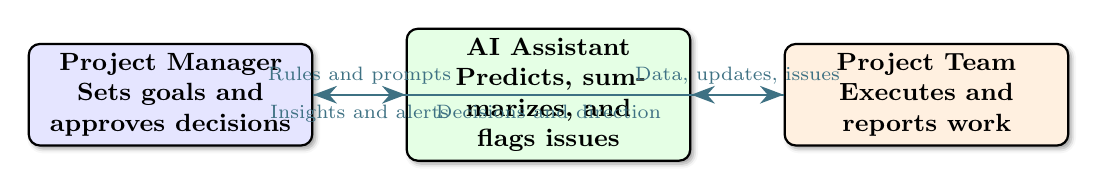
\begin{tikzpicture}[
  rolebox/.style={rectangle, draw, thick, rounded corners=4pt, minimum width=3.6cm, text width=3.2cm, minimum height=1.1cm, align=center, font=\small\bfseries,
    blur shadow={shadow blur steps=3, shadow xshift=0.4mm, shadow yshift=-0.4mm}},
  arr/.style={-{Stealth[length=3mm]}, thick, primary!80}
]
  \node[rolebox, fill=blue!10] (manager) at (0,0) {Project Manager\\Sets goals and approves decisions};
  \node[rolebox, fill=green!10] (ai) at (4.8,0) {AI Assistant\\Predicts, summarizes, and flags issues};
  \node[rolebox, fill=orange!12] (team) at (9.6,0) {Project Team\\Executes and reports work};

  \draw[arr] (manager) -- node[above, font=\scriptsize] {Rules and prompts} (ai);
  \draw[arr] (team) -- node[above, font=\scriptsize] {Data, updates, issues} (ai);
  \draw[arr] (ai) -- node[below, font=\scriptsize] {Insights and alerts} (manager);
  \draw[arr] (manager) -- node[below, font=\scriptsize] {Decisions and direction} (team);
\end{tikzpicture}
\end{center}

\subsection{Benefits and Limits}

\begin{longtable}{p{5.8cm}p{5.8cm}}
\toprule
\textbf{Potential Benefits} & \textbf{Practical Limits} \\
\midrule
Faster reporting and summarization & Poor results when input data is incomplete or noisy \\
Earlier detection of schedule and cost risk & Models may inherit bias from past project history \\
Better visibility into team workload & AI can recommend actions without understanding organizational politics \\
Improved consistency in documentation & Sensitive project data may raise privacy or compliance concerns \\
Automation of repetitive coordination tasks & Final accountability still belongs to human managers \\
\bottomrule
\end{longtable}

%=============================================================
\section{AI Across Planning, Execution, and Control}
%=============================================================

\subsection{AI in Planning}

\begin{itemize}[leftmargin=*]
  \item Generate draft work breakdown structures from project objectives.
  \item Suggest milestones, dependencies, and probable delivery dates.
  \item Estimate effort by comparing the current project to similar historical projects.
  \item Identify missing requirements or ambiguous scope statements from project documents.
\end{itemize}

\subsection{AI in Execution}

\begin{itemize}[leftmargin=*]
  \item Summarize stand-up meetings and extract action items.
  \item Recommend task assignments based on skill patterns and availability.
  \item Prioritize backlog items using urgency, impact, and dependency signals.
  \item Monitor project communication streams for blockers, escalation signals, or unresolved issues.
\end{itemize}

\subsection{AI in Monitoring and Control}

\begin{itemize}[leftmargin=*]
  \item Predict whether milestones will be missed.
  \item Detect cost variance trends earlier than manual review.
  \item Analyze defect patterns and quality risk indicators.
  \item Produce dashboard narratives in plain language for managers and stakeholders.
\end{itemize}

\begin{examplebox}[Simple AI PM Workflow]
A team uses issue tracker data, sprint velocity, meeting transcripts, and timesheet summaries as inputs. An AI service generates a weekly report that highlights late tasks, probable schedule slippage, unresolved risks, and missing approvals. The project manager reviews the output before sharing it with stakeholders.
\end{examplebox}

%=============================================================
\section{Agile, Scrum, and Hybrid AI-Supported Delivery}
%=============================================================

\subsection{Why Agile Fits Many IT Projects}

\begin{conceptbox}[Adaptive Delivery]
Many IT projects, especially software and analytics projects, face changing requirements. Agile methods address this by delivering incrementally, gathering feedback frequently, and re-plioritizing based on value and learning.
\end{conceptbox}

\subsection{Common Agile Roles and Artifacts}

\begin{longtable}{p{2.8cm}p{3.7cm}p{5.0cm}}
\toprule
\textbf{Element} & \textbf{Purpose} & \textbf{AI Support Example} \\
\midrule
Product backlog & Ordered list of desired work & Suggest item grouping, deduplicate similar stories \\
Sprint backlog & Work selected for current sprint & Flag overload based on historical velocity \\
Scrum Master & Removes blockers and supports process & Summarize impediments across stand-ups \\
Product Owner & Prioritizes value and requirements & Analyze feedback themes from users or stakeholders \\
Burndown chart & Visualizes remaining work & Add natural-language explanation of trend anomalies \\
\bottomrule
\end{longtable}

\subsection{Hybrid Project Management}

\begin{itemize}[leftmargin=*]
  \item Some parts of a project may need predictive planning, such as procurement, security review, or compliance milestones.
  \item Other parts may need Agile iteration, such as interface design, analytics features, or integration refinement.
  \item AI can support both by improving forecasts, summarizing progress, and highlighting deviations.
\end{itemize}

\begin{alertbox}[Managerial Caution]
AI recommendations should not be treated as unquestionable truth. If the backlog is poorly written, if stakeholders change their minds, or if the team composition shifts, an AI-generated sprint plan can become misleading very quickly.
\end{alertbox}

%=============================================================
\section{Data, Metrics, and Dashboards for AI Project Management}
%=============================================================

\subsection{What Data AI Needs}

\begin{itemize}[leftmargin=*]
  \item Historical schedules and milestone completion data.
  \item Task durations, effort logs, and velocity records.
  \item Risk registers, issue logs, and change requests.
  \item Meeting notes, chat summaries, and decision records.
  \item Quality indicators such as defects, rework, and test outcomes.
\end{itemize}

\subsection{Important Performance Metrics}

\begin{longtable}{p{3.2cm}p{3.5cm}p{4.8cm}}
\toprule
\textbf{Metric} & \textbf{What It Shows} & \textbf{AI Use} \\
\midrule
Schedule variance & Difference between planned and actual timeline & Predict future delay risk \\
Cost variance & Difference between budgeted and actual cost & Flag overspending patterns \\
Velocity & Team delivery rate in Agile work & Forecast sprint capacity \\
Defect density & Quality problems relative to output size & Identify unstable modules or teams \\
Lead time & Time from request to completion & Detect bottlenecks in workflow \\
\bottomrule
\end{longtable}

\subsection{Dashboard Design Principles}

\begin{itemize}[leftmargin=*]
  \item Show only the most decision-relevant indicators.
  \item Use trends and comparisons, not raw counts alone.
  \item Separate confirmed issues from AI-predicted risks.
  \item Keep audit trails so managers can explain why a recommendation was generated.
\end{itemize}

\subsection{Interpretability Matters}

\begin{conceptbox}[Explainable Insight]
If an AI system predicts that a project will miss its deadline, the project manager should know why. Useful explanations might include reduced team velocity, late approvals, unresolved blockers, increasing defect count, or repeated scope changes.
\end{conceptbox}

%=============================================================
\section{Risk, Governance, and Ethics in AI-Based Project Management}
%=============================================================

\subsection{Project Risks Introduced by AI}

\begin{itemize}[leftmargin=*]
  \item Overreliance on AI-generated estimates.
  \item Leakage of confidential project data into external tools.
  \item Biased recommendations caused by poor historical data.
  \item Hallucinated summaries or inaccurate status interpretations.
  \item False confidence in automated prioritization.
\end{itemize}

\subsection{Governance Controls}

\begin{itemize}[leftmargin=*]
  \item Define which project data AI tools are allowed to access.
  \item Keep a human approval step for major decisions.
  \item Review prompt templates, model behavior, and security controls regularly.
  \item Log outputs that affect budget, schedule, scope, or staffing decisions.
  \item Train teams to challenge AI outputs instead of blindly accepting them.
\end{itemize}

\subsection{Ethical Questions}

\begin{itemize}[leftmargin=*]
  \item Is the AI making recommendations that unfairly favor or penalize certain team members?
  \item Is the system using personal productivity data in ways employees did not expect?
  \item Are stakeholders clearly informed when reports or summaries are AI-generated?
  \item Can a project team explain and justify a decision that was influenced by AI?
\end{itemize}

\begin{alertbox}[Principle of Accountability]
AI may assist with analysis, but responsibility for project outcomes stays with human managers and sponsoring organizations. Accountability cannot be delegated to a model.
\end{alertbox}

%=============================================================
\section{Case Study and BSIT Skills Roadmap}
%=============================================================

\subsection{Mini Case Study: AI-Supported Student Information System Project}

\begin{examplebox}[Scenario]
A BSIT team is assigned to build a student information dashboard for a university. The team uses Agile delivery with two-week sprints. An AI assistant helps draft user stories, summarize sprint reviews, detect repeated blockers from stand-up notes, and forecast whether the final release date is at risk.
\end{examplebox}

\textbf{Project management lessons from the case:}
\begin{itemize}[leftmargin=*]
  \item Human leaders still define scope, approve priorities, and resolve tradeoffs.
  \item AI speeds up reporting and surfacing risk, but team data quality determines usefulness.
  \item Sensitive student data requires strong governance over AI tools and logs.
  \item The most useful AI outputs are often summaries, risk signals, and planning suggestions rather than full automation.
\end{itemize}

\subsection{Skills BSIT Students Should Build}

\begin{multicols}{2}
\begin{itemize}[leftmargin=1.2em]
  \item Project charter writing
  \item Work breakdown structuring
  \item Gantt and sprint planning
  \item Risk register design
  \item Dashboard interpretation
  \item Prompting AI assistants responsibly
  \item Data privacy awareness
  \item Team communication and reporting
\end{itemize}
\end{multicols}

\subsection{Professional Mindset}

\begin{conceptbox}[AI as Decision Support]
The best project managers do not ask AI to think for them. They use AI to surface patterns faster, reduce manual reporting effort, and improve visibility while keeping control over judgment, ethics, communication, and accountability.
\end{conceptbox}

%=============================================================
\section{Key Takeaways and Review Questions}
%=============================================================

\subsection{Key Takeaways}

\begin{itemize}[leftmargin=*]
  \item IT project management organizes technology work so it can be delivered with control over scope, time, cost, quality, and risk.
  \item AI can strengthen planning, forecasting, reporting, and risk detection across the project lifecycle.
  \item Good data, human oversight, and governance are necessary for AI-based project management to be trustworthy.
  \item Agile and hybrid delivery models can benefit from AI-supported summaries, predictions, and prioritization assistance.
  \item BSIT students should learn both classical project management foundations and responsible use of AI tools.
\end{itemize}

\subsection{Review Questions}

\begin{enumerate}[leftmargin=*]
  \item What is the difference between a project and ongoing operations?
  \item How can AI improve planning and monitoring in IT projects?
  \item Why should managers be cautious about AI-generated estimates and recommendations?
  \item What kinds of project data are useful for AI-based forecasting?
  \item How can Agile teams use AI without giving up human control?
  \item Why is governance necessary when AI tools process project information?
\end{enumerate}

\begin{examplebox}[Short Reflection Task]
Imagine that your BSIT class is developing a campus mobile application. Describe one way AI could help during planning, one way it could help during execution, and one governance rule you would apply before letting the AI analyze project data.
\end{examplebox}

\vfill
\begin{center}
{\large\textcolor{primary}{\textbf{End of Handout}}}\\[4pt]
{\small\textcolor{gray!70!black}{IT Project Management --- BSIT Program}}
\end{center}

\end{document}